\documentclass{pre-tfg}
\usepackage{custom}

\title{\REDNOTE{Título del TFG}}% TODO
\author{José Ángel Martín Baos}
\advisorFirst{Dr. Luis Rodríguez Benítez}
\advisorDepartment{Tecnologías y Sistemas de Información}
\advisorSecond{Dr. Ricardo Garcia Rodenas}
\intensification{Ingeniería de Computadores}
\docdate{2018}{February}


\begin{document}

\maketitle
\tableofcontents

\newpage


\section{INTRODUCTION} % TODO
%1. Enmarcar el problema. Necesidad de ciudades inteligentes que se anticipen a la contaminación y tomen medidas paliativas (Restringir el tráfico [por número vehiculos, matricula, calles...]).

Urban vehicle traffic is often the main source of air pollution in urban areas, with detrimental
effects on local air quality, ecology, and human health. Therefore, there is an increasing
need to estimate precisely the contribution of road transport to air pollution in the
cities, so that pollution-reduction measures (such as emission standards, traffic management,
Intelligent Transportation Systems (ITS) or Dynamic Traffic Management (DTM) systems)
can be designed and implemented appropriately \cite{SNB10}. These pollution-reduction measures
are becoming increasingly relevant due to the continued growth in vehicle use and the
deterioration in driving conditions (congestion). Many authorities find it difficult to meet
their environmental targets (e.g. air quality standards or national emission ceilings) and,
therefore, reliable emissions models are needed, in order to predict accurately the road transport
contribution to air pollution.

Therefore, intelligent cities are needed to prevent situations of high level of contamination in the cities and take measures when these situations occur. These cities must predict the pollution peaks and take palliative measures, such as restrict the traffic by the number of vehicles, by the license plates, close traffic in some streets, etc. Moreover, traffic flows must be measured and controlled, as they will affect to the pollution levels on that city. For this reason, those cities must relay in an IoT (Internet of Things) infrastructure that supports the those systems, as well as sensor-based big data applications \cite{Bib18}.


%2. Todo esto requiere de una infraestrucutra técnologica que le de soporte. Ciudades son entornos distribuidos, tiempo real, masivo.
% Se necesita una arquitectura distribuida que controle la contaminación por zonas/Calles, a diferencia de los sistemas actuales.

Typical pollution surveillance and control systems are composed by big and expensive devices that are only located in some points in a city, hence, they provide information for vast areas and sometimes those systems are not scalable. However, cities are distributed environments, where the events occur in real time and in a massive way. Therefore, a cheap distributed IoT architecture is needed to control pollution levels by zones or streets. These can be combined with a traffic surveillance system in order to have a complete system that can be used as a Decision Support System (DSS) to help authorities to take decisions about environmental problems caused by pollution before they occur.

%3. El objetivo del TFG es hacer un prototipo de este sistema. Se centraría unicamente en la estructura que daría soporte a un sistema inteligente (que no se aborda en este TFG).
The objective in this Bachelor of Science Thesis (BSc. thesis from now on) is to design and build a prototype of the previous system. It will be focus only in the design and implementation of the software and hardware architecture that can be used as a base for the developing of an intelligent system for predicting pollution levels and proceed according to them. A cheap embedded system will be used for designing the architecture in order to get a scalable system.



\section{SPECIFIC TECHNOLOGY COURSED}

The Table \ref{tab:tec-especifica} shows the specific technology coursed (\emph{Ingeniería de Computadores}). In addition, Table \ref{tab:competencias} shows the different specific competences that are addressed in this BSc. thesis. 

\begin{table}[hp]
	\centering
	\caption{Specific technology coursed}
	\label{tab:tec-especifica}
	
	\zebrarows{1}
	\begin{tabular}{cp{0.32\textwidth}}
		\hline
		&Tecnologías de la Información \\
		&Computación \\
		&Ingeniería del Software \\
		\textbf{X}&Ingeniería de Computadores \\
		\hline
	\end{tabular}
\end{table}

\begin{table}[hp]
  \centering
  \caption{Justification of the specific competences addressed in this BSc. thesis}
  \label{tab:competencias}

  \zebrarows{1}
  \begin{tabular}{m{0.06\linewidth}m{0.4\linewidth}m{0.01\linewidth}m{0.46\linewidth}}
    &\textbf{Competency} && \textbf{Justification} \\
    \hline

    \textbf{[IC1]}& Ability to design and build digital systems, including computers, microprocessor-based systems and communications systems.&& In this BSc. thesis a microprocessor-based system is going to be developed using a Raspberry Pi. \\
    
    \textbf{[IC2]}& Ability to develop specific processors and embedded systems, as well as to develop and optimize the software of that systems.&& In this BSc. thesis some software code has to be developed and optimized in order to execute in real time on the Raspberry Pi. \\
    
    \textbf{[IC4]}& Ability to design and implement system and communications software.&& Some system software must be developed in order to control de device as well as a communication software to send the different data to the servers. \\
    
    \textbf{[IC5]}& Ability to analyse, evaluate and select the most appropriate hardware and software platforms to support embedded and real-time applications.&& In this BSc. thesis the most convenient real-time embeded system platform must be selected to implement the desired functionality. \\
    
    \textbf{[IC7]}& Ability to analyse, evaluate, select and configure hardware platforms for the development and execution of applications and computer services.&& In this BSc. thesis the most convenient hardware platforms must be selected and configured to implement the sensors as well as to process the different data collected by those sensors. \\
    
    \hline
  \end{tabular}
\end{table}


\section{OBJECTIVES}

The main objective of this BSc. thesis is the analysis, design and implementation of a cheap distributed architecture based on Raspberry Pi embedded systems to monitor and obtain data about the pollution level, in conjunction with traffic flows information on several points of a city in real time. This objective is expected to be fulfilled through the achievement of the following partial sub-objectives:

\begin{table}[!h]
	\centering
	\caption{Sub-objectives of the BSc. thesis}
	\label{tab:sub-objectives}
	
	\zebrarows{1}
	\begin{tabular}{m{0.05\linewidth}m{0.8\linewidth}}
		\textbf{ID} & \textbf{Objective} \\
		\hline
		
		\textbf{O.1}& Develop a module to calculate the flow of vehicles using the Raspberry Pi Camera.  \\
		
		\textbf{O.2}& Develop a module to obtain environmental parameters on the Raspberry Pi System.  \\
		
		\textbf{O.3}& Develop a sever and a module to synchronize the data of the Raspberry Pi modules with that server.  \\
		
		\textbf{O.4}& Develop a program to monitor the data recorded by the different Raspberry Pi systems in real time and control them.  \\
		
		\textbf{O.5}& \REDNOTE{------------------------------------------------------------}  \\
		
		\hline
	\end{tabular}
\end{table}


\section{\REDNOTE{METHODOLOGIES AND WORK PHASES}}

In the last few years, the number of companies, with different size and from different areas, using agile development methodologies has increased considerably. These methodologies are not only used by the software development companies, but also they are used by a wide range of companies. In the software engineering field, agile methodologies gain a lot of importance due to the complexity sometimes needed to specify the different requirements of a product in an unique phase. Agile methodologies makes a great difference with respect to \emword{Waterfall} model where carrying out a change once the product is almost finished is very costly.

In an agile project it is sought to divide the tasks of the software project in increments with a minimum planning and a short duration (normally between one and four weeks). Each iteration produces an operational prototype that is revised together with the client. Therefore, we can affirm that the life cycle of the agile methodologies is iterative and incremental.

In our view, Scrum fits nicely with the problem dealt in this BSc. thesis as this project consist on a hardware-software system organised in several stages. Furthermore, as consequence of being one of the most used agile methodologies, lot of literature has been written about it, for this reason, Scrum has been chosen. Specifically, Scrum methodology \cite{ScrumGuide} will be adapted to an one-person development. To manage the progress of the project graphically the Kanban technique with the tool Trello will be used.

Scrum has two main characteristics: The first one is that the development of the software is carried out in incremental iterations, whilst the second one is that coordination meetings are held throughout the project. In Scrum, the product is developed in series with a duration from one to four weeks called \emword{sprints}. The different requirements are captured as elements of a list called \emword{product backlog} which is created at the beginning of the project. Figure \ref{fig:5-ScrumSprints} represents the complete Scrum life cycle.

\begin{figure}[!h]
	\begin{center}
		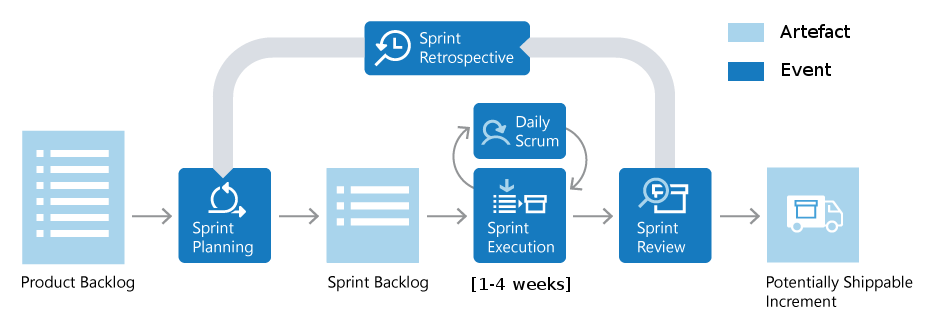
\includegraphics[width=1\textwidth]{ScrumSprints-v2.png}	
		\caption{Scrum life cycle}{Source: \url{https://www.visualstudio.com/es/learn/what-is-scrum}}
		\label{fig:5-ScrumSprints}
	\end{center}
\end{figure}

Kanban \cite{Gar11,KS10} is a Japanese technique for managing the progress of the project. It was invented by Toyota and was used to control the progress of their work in the production line. Therefore, Kanban is not a specific software development technique, nevertheless, in the last few years it has been used in the management of software projects.

Kanban allows the development team to visualize the workflow of the different tasks. Normally, consists in using a slate board with three columns: \emph{To Do}, \emph{Doing} and \emph{Done}, that represents the different phases a task passes until it is completed. Each task in which a sprint is divided is considered as a card which is put into the slate board. An example of this concept can be seen in Figure \ref{fig:5-KanbanBoard}.

To manage the Kanban Board, Trello is used, as it was previously indicated. This tool allows the creation of several boards. In each board many columns can be created with various tasks that can be moved from one column to another by means of a very friendly interface.

\begin{figure}[!h]
	\begin{center}
		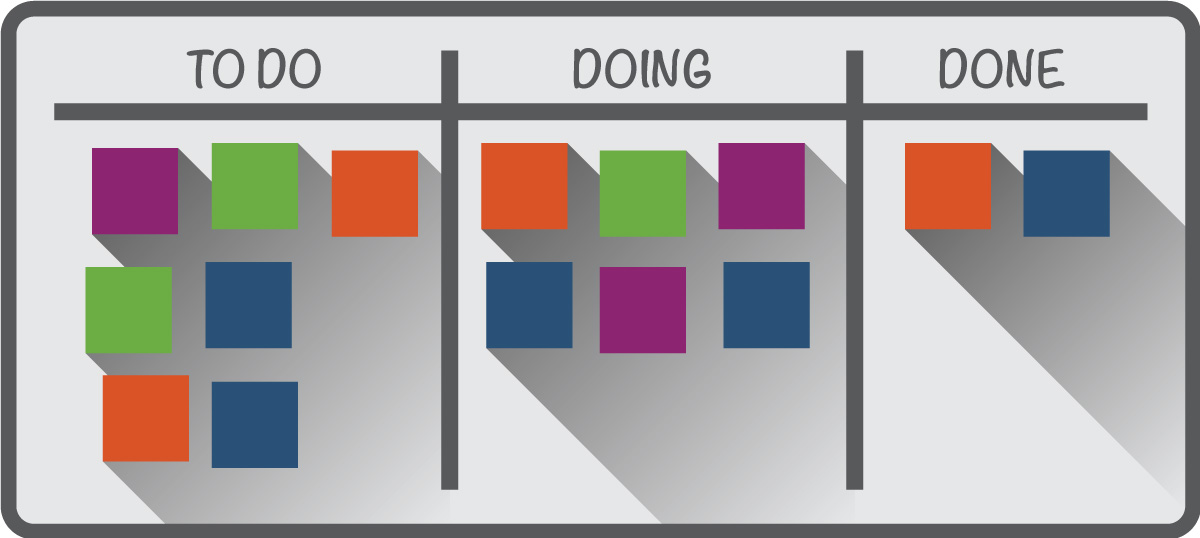
\includegraphics[width=0.8\textwidth]{KanbanBoard.jpg}
		\caption{Kanban Board}
		\label{fig:5-KanbanBoard}{Source: \url{www.qe2ingenieria.com}}
	\end{center}
\end{figure}

The development methodology is used by developers and engineers to write code, helping them in the process and giving some guidelines when developing computer systems in order to maintain a high code quality. The development methodology used is \REDNOTE{ XXX }

\REDNOTE{...}



\REDNOTE{Based on the sub-objectives established in Table \ref{tab:sub-objectives}, the following project plan is proposed, as shown in Table \ref{tab:Sprints}.}

\begin{table}[!h]
	\centering
	{\small
		\begin{tabular}{|P{.08\textwidth}p{.56\textwidth}P{.15\textwidth}P{.08\textwidth}|}
	\hline
	\rowcolor{tabheadbg}
	\multicolumn{4}{|c|}{\textscale{.8}{\textbf{Sprints}}} \\
	\hline
	\hline
	\textscale{.8}{\textbf{Sprint}}			& \textscale{.8}{\textbf{Name}}	& \textscale{.8}{\textbf{User stories}}	& \textscale{.8}{\textbf{Estimate}} \\
	\hline
	0 	& Initial planning		 	& - 	& 35h \\ 
	\hline
	1 	& Development a basic algorithm to calculate the flow of vehicles		 		 	& 1, 2, 3 	& 50h \\ 
	\hline
	2 	& Design of an environmental parameters monitoring system		 	& \REDNOTE{...} 	& \REDNOTE{X}h \\ 
	\hline

\end{tabular}
	}
	\caption{Sprints}
	\label{tab:Sprints}
\end{table}



\section{RESOURCES THAT ARE INTENDED TO BE USED}

In this section we are going to describe the different technologies that are intended to be employed during the development of this BSc. thesis.

\subsection{Hardware resources}
Now, the different hardware resources intended to be used in the BSc. thesis are detailed. These include the computer that will be used to develop the BSc. thesis, the Raspberry Pi and the different peripherals attached to it.

\begin{itemize}
	\item \emlst{Development computer.} The personal computer of the student will employ for this purpose. The spec table is shown in Table \ref{tab:development-computer-spec-table}.
	
	\begin{table}[!h]
		\centering
		{\small
			\begin{tabular}{ |l|l|}
	\hline
	\rowcolor{tabheadbg}
	\multicolumn{2}{|c|}{\textscale{.8}{\textbf{Development computer (\emph{draco}) specs}}} \\
	\hline
	Model						& Asus Zeenbook UX430UA \\
	\hline
	Processor					& Intel® Core™ i7-7500U CPU at 2.70GHz $\times$ 4 \\
	\hline
	RAM memory 					& 8 GB \\
	\hline 
	Hard drive					& 512 GB HDD \\
	\hline
	First Operating System		& Ubuntu 16.04.3 LTS \\
	\hline
	Second Operating System		& Windows 10 \\
	\hline

\end{tabular}
		}
		\caption{Development computer spec table}
		\label{tab:development-computer-spec-table}
	\end{table}
	
	\item \emlst{Raspberry Pi 3.} The Raspberry Pi is a low cost, credit-card sized computer. The Raspberry Pi 3 is the third-generation Raspberry Pi. Table \ref{tab:raspberry-pi3-spec-table} shows its spec table. With this computer a memory card is also needed. The one used is the \emph{Samsung SDHC EVO 8gb Class 10+}.
	
	\begin{table}[!h]
		\centering
		{\small
			%\begin{tabular}{ |l|l|l|}
%	\hline
%	\rowcolor{tabheadbg}
%	\multicolumn{3}{|c|}{\textscale{.8}{\textbf{Raspberry Pi 3 Model B specs}}} \\
%	\hline
%	Price						& $\sim$35\euro{} \\
%	\hline
%	SoC							& Broadcom BCM2837 \\
%	\hline
%	Processor					& Quad Core ARM Cortex A53 (ARMv8) at 1.2GHz 64bit \\
%	\hline
%	RAM memory 					& 1 GB \\
%	\hline 
%	GPIO pins					& 40 \\
%	\hline
%	\multirow{7}{*}{External ports}
%		& HDMI \\ 
%		& CSI camera port \\ 
%		& DSI display port \\ 
%		& Micro SD port \\
%		& 4 $\times$ USB 2 ports \\
%		& Ethernet port \\
%		& Audio jack 3,5 mm \\
%	\hline
%	\multirow{2}{*}{Wireless connections}
%	& BCM43438 wireless LAN  \\ 
%	& Bluetooth Low Energy (BLE) \\
%	\hline
%
%\end{tabular}

\begin{tabular}{ |l|l|l|}
	\hline
	\rowcolor{tabheadbg}
	\multicolumn{3}{|c|}{\textscale{.8}{\textbf{Raspberry Pi 3 Model B specs}}} \\
			\hline
	Price                                 & $\sim$35\euro{}                                  & \multirow{14}{*}{
		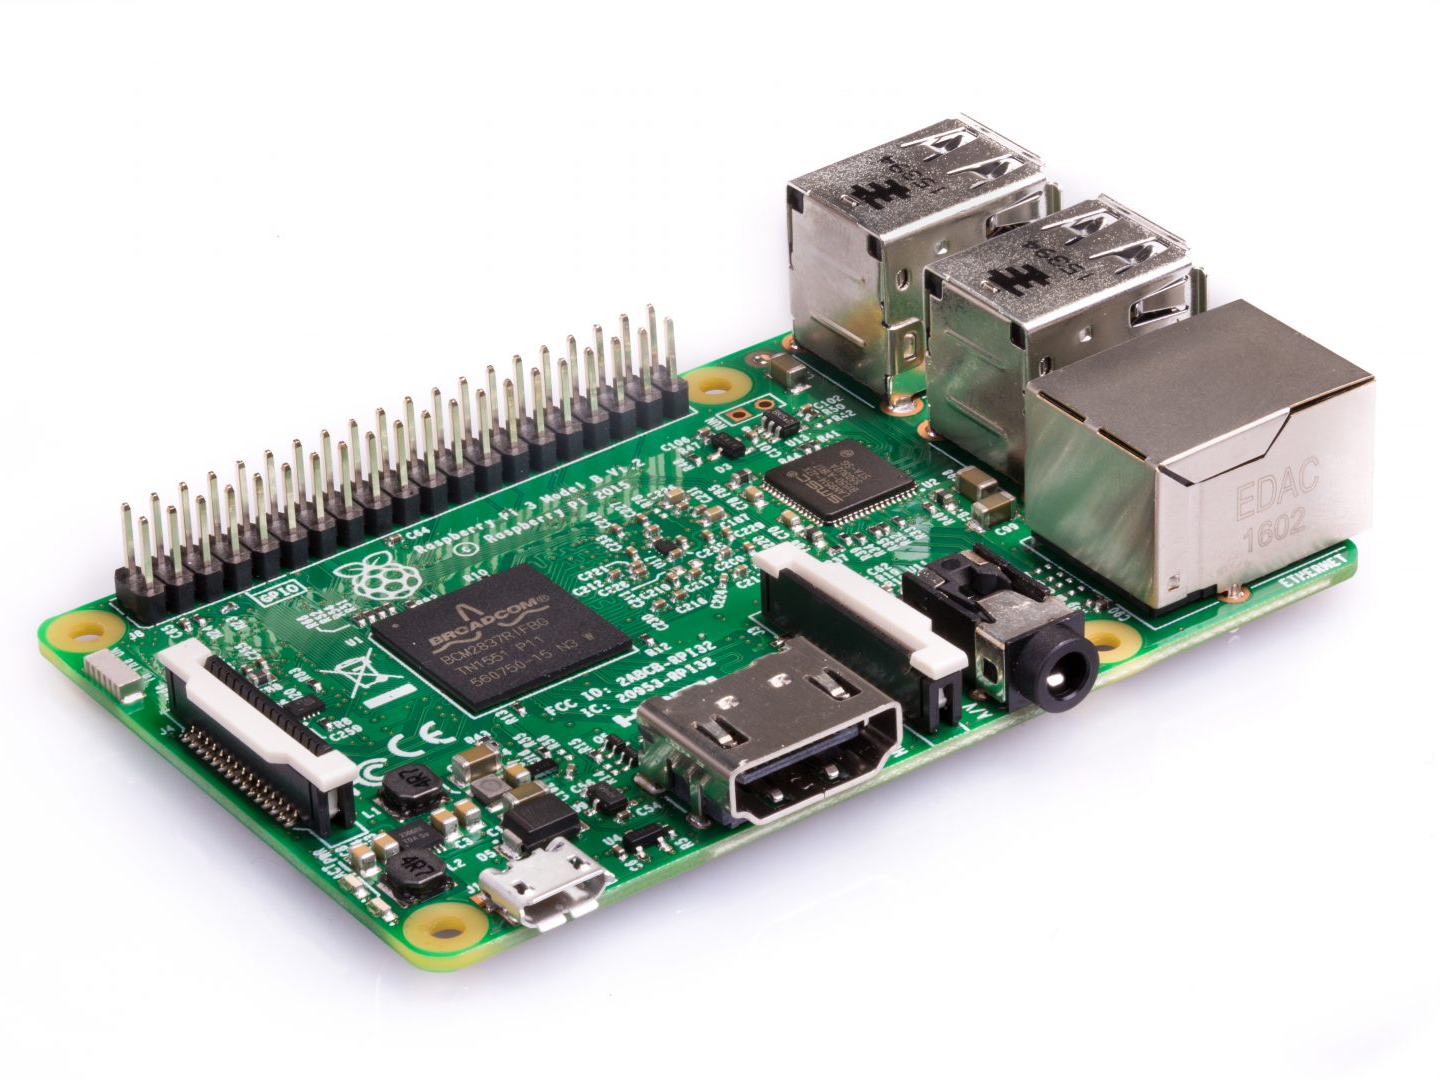
\includegraphics[width=0.36\textwidth]{5-RaspberryPi3.jpg}
	} \\ \cline{1-2}
	SoC                                   & Broadcom BCM2837                                 &                         \\ \cline{1-2}
	Processor                             & Quad Core ARM Cortex A53 				 &                         \\ 
			                              & (ARMv8) at 1.2GHz 64bit 								 &                         \\ \cline{1-2}
	RAM memory                            & 1 GB                                             &                         \\ \cline{1-2}
	GPIO pins                             & 40                                               &                         \\ \cline{1-2}
	\multirow{7}{*}{External ports}       & HDMI                                             &                         \\
	& CSI camera port                                  &                         \\
	& DSI display port                                 &                         \\
	& Micro SD port                                    &                         \\
	& 4 × USB 2 ports                                  &                         \\
	& Ethernet port                                    &                         \\
	& Audio jack 3,5 mm                                &                         \\ \cline{1-2}
	\multirow{2}{*}{Wireless connections} & BCM43438 wireless LAN                            &                         \\ \cline{2-2}
	& Bluetooth Low Energy (BLE)                       &                         \\ \hline
	
	
\end{tabular}

		}
		\caption{Raspberry pi 3 spec table}
		\label{tab:raspberry-pi3-spec-table}
	\end{table}
	
	\item \emlst{Raspberry Pi Camera Module V2 \cite{PiCameraDoc}.} It is a hardware module that allows the Raspberry Pi to capture pictures and record videos using the CSI port. The camera that will be used is the \emph{PI NOIR CAMERA V2}.\footnote{More information in https://www.raspberrypi.org/products/pi-noir-camera-v2/} The table \ref{tab:raspberry-pi3-camera-specs} shows its specs. \label{itm:Pi-camera-module-v2}
	
	\begin{table}[!h]
		\centering
		{\small
			%\begin{tabular}{ |l|l|}
%	\hline
%	\rowcolor{tabheadbg}
%	\multicolumn{2}{|c|}{\textscale{.8}{\textbf{Pi NoIR Camera V2 specs}}} \\
%	\hline
%	Price						& $\sim$25\euro{} \\
%	\hline
%	Weight						& 3g \\
%	\hline
%	Resolution					& 8 Megapixels \\
%	\hline 
%	Dimensions					& 25$\times$24$\times$9 mm \\
%	\hline	
%	Sensor						& Sony IMX219 \\
%	\hline
%	\multirow{3}{*}{Video modes}
%		& 1080$\times$120p at 30 fps \\ 
%		& 720$\times$480p at 60 fps\\ 
%		& 640$\times$480p at 60$/$90 fps \\ 
%	\hline
%	Additional information		& No Infrared filter (NoIR) \\
%	\hline
%\end{tabular}

% Please add the following required packages to your document preamble:
% \usepackage{multirow}


\begin{tabular}{|l|l|l|}
	\hline
	\rowcolor{tabheadbg}
	\multicolumn{3}{|l|}{\textscale{.8}{\textbf{Pi NoIR Camera V2 specs}}}                       \\ \hline
	Price                        & $\sim$25\euro{}                     & \multirow{9}{*}{
		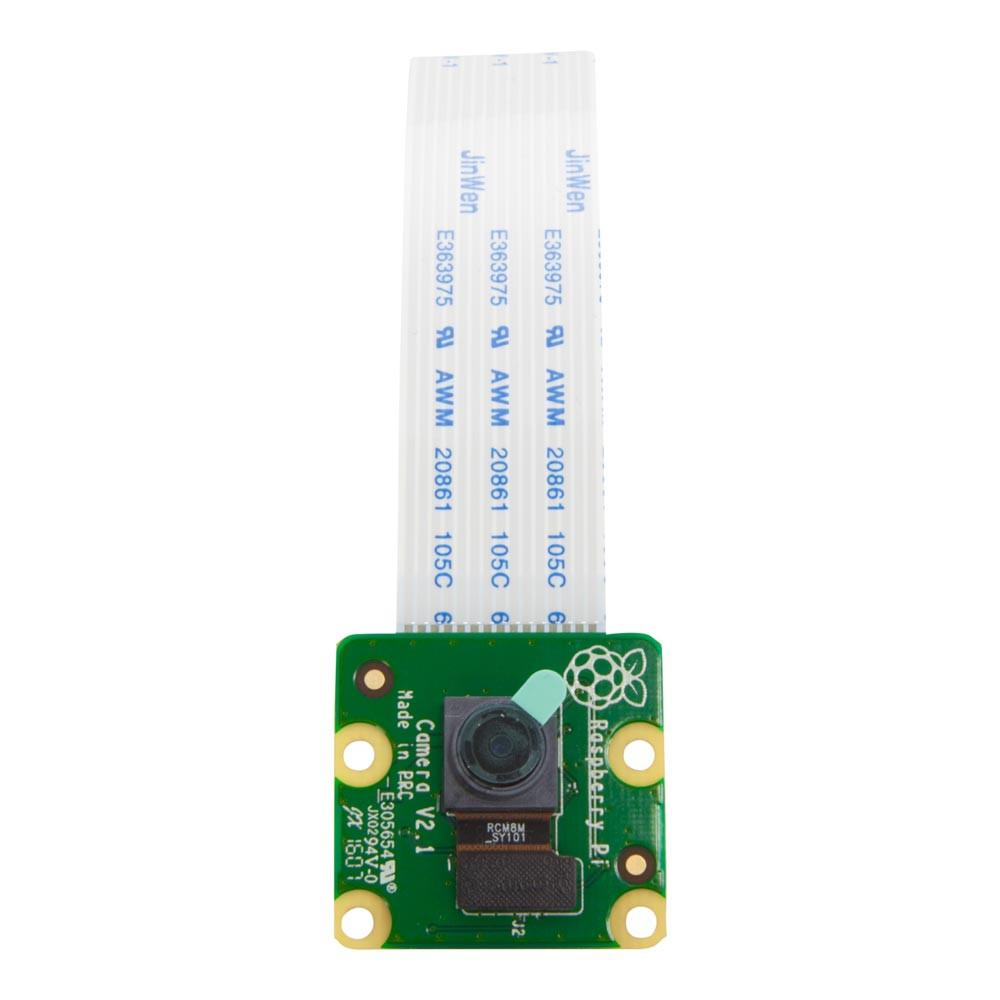
\includegraphics[width=0.28\textwidth]{5-PiCamera.jpg}
	} \\ \cline{1-2}
	Weight                       & 3g                        &                   \\ \cline{1-2}
	Resolution                   & 8 Megapixels              &                   \\ \cline{1-2}
	Dimensions                   & 25×24×9 mm                &                   \\ \cline{1-2}
	Sensor                       & Sony IMX219               &                   \\ \cline{1-2}
	\multirow{3}{*}{Video modes} & 1080p at 30 fps           &                   \\
	& 720p at 60 fps            &                   \\
	& 640x480p at 60/90 fps     &                   \\ \cline{1-2}
	Additional information       & No Infrared filter (NoIR) &                   \\ \hline
\end{tabular}
		}
		\caption{Pi NoIR Camera V2 spec table}
		\label{tab:raspberry-pi3-camera-specs}
	\end{table}
	
	\item \emlst{Sense HAT \cite{SenseHAT}.} It is an add-on board which is placed on top of the Raspberry Pi board. It was made for the Astro Pi mission which took place in December 2015. This board is composed by several components: 8x8 RGB LED matrix, five-button joystick and some sensors (temperature, humidity, barometric pressure, magnetometer, accelerometer and gyroscope).
	
	\item \emlst{Power bank battery.} The Raspberry Pi board is going to be powered using a power bank battery.
	
	\item \emlst{MQ-7 Sensor. \cite{MQ7}} This sensor is able to measure Carbon Monoxide (CO) concentrations in the air. The MQ-7 can detect concentrations anywhere from 20 to 2000 ppm (parts per million) and has a fast response time. This sensor works with an input voltage of 5 volts and provide an analog output, therefore an anaglog to digital converter is needed.
	
	\item \emlst{MQ-2 Sensor \cite{MQ2}.} This sensor is able to measure methane, butane, petroleum gas and smoke in concentrations between 300 to 10000 ppm. As the previous sensor, this one also works with a voltage of 5 volts and provide an analog output.
	
	\item \emlst{Analog-to-digital-converter \cite{ADC}.} Ananalog-to-digital converter (ADC) is a system that converts an analog signal into a digital signal. Therefore, the input analog current is converted to a digital number proportional to the magnitude of the current that can be understood by a digital system.	
	
\end{itemize} 



\subsection{Software resources}
The different software resources that will be employed are described. These include the Operating System, programming languages, libraries, the different development tools and the software that will be used to generate the documentation.

\textbf{Operating Systems:}
\begin{itemize}
	\item \emlst{Ubuntu 16.04.3 LTS.}
	\item \emlst{Debian 9 “Stretch”.}
	\item \emlst{Raspbian.}
\end{itemize}

\textbf{Programming Languages:}
\begin{itemize}
	\item \emlst{Python 3 \cite{Dow12}.} Python is a high-level programming language.  Python will be used because it has lot of support for Raspberry Pi.
	
\end{itemize}

\textbf{Libraries:}
\begin{itemize}
	\item \emlst{Python PiCamera \cite{PiCameraDoc}.} Python library that provides an interface for controlling the Raspberry Pi camera.
	
	\item \emlst{Python NumPy \cite{NumPy}.} NumPy is a open-source scientific computing package for Python.
	
	\item \emlst{Python Matplotlib \cite{Hun07}.} Matplotlib is a Python 2D plotting library which produces quality figures in a variety of formats.
	
\end{itemize}

\textbf{Development tools:}
\begin{itemize}
	\item \emlst{Atom.} Atom is a free open-source text and source coder editor for macOS, Linux and Windows developed by GitHub.
	
	\item \emlst{Vi.} Vi is a console text editor originally created for the Unix  Operating System. 
	
	\item \emlst{Git \cite{CS14}.} Git is a version control system for tracking changes in computer files and coordinating work on those files among multiple people.
	
	\item \emlst{GitHub.} GitHub is a web-based Git version control repository.
	
	%\item \textbf{Make}    https://www.gnu.org/doc/doc.html
	
	
\end{itemize}

\textbf{Software used for the documentation:}
\begin{itemize}
	\item \emlst{Trello.} Trello is a web tool which provides support for the Kanban technique allowing to manage the progress of the project.
	
	\item \emlst{\LaTeX{} \cite{Kot11}.} \LaTeX{} is a software for typesetting documents.
	
	\item \emlst{TeXstudio.} TeXstudio is a cross-platform and open source \LaTeX{} editor.
	
	\item \emlst{esi-tfg \LaTeX{} class.} It is a \LaTeX{} class with allows to write the BSc. thesis in a simple way, as its format conforms to the specification established for the BSc.
	
	\item \emlst{GIMP.} GIMP (GNU Image Manipulation Program) is a free and open-source raster graphics editor used for image editing.
	
	%\item \textbf{Inkscape.}
	
\end{itemize}


%\bibliographystyle{alpha}
\bibliographystyle{plain}
\singlespacing
\bibliography{main}


\end{document}


% Local Variables:
% coding: utf-8
% mode: flyspell
% ispell-local-dictionary: "castellano8"
% mode: latex
% End:
